\documentclass[journal,10pt,twocolumn]{article}
\usepackage{graphicx}
\usepackage[margin=0.5in]{geometry}
\usepackage[cmex10]{amsmath}
\usepackage{array}
\usepackage{booktabs}
\usepackage{mathtools}
\title{\textbf{Conic section Assignment}}
\author{Divya Sai }
\date{November 2022}


\providecommand{\norm}[1]{\left\lVert#1\right\rVert}
\providecommand{\abs}[1]{\left\vert#1\right\vert}
\let\vec\mathbf
\newcommand{\myvec}[1]{\ensuremath{\begin{pmatrix}#1\end{pmatrix}}}
\newcommand{\mydet}[1]{\ensuremath{\begin{vmatrix}#1\end{vmatrix}}}
\providecommand{\brak}[1]{\ensuremath{\left(#1\right)}}
\providecommand{\lbrak}[1]{\ensuremath{\left(#1\right.}}
\providecommand{\rbrak}[1]{\ensuremath{\left.#1\right)}}
\providecommand{\sbrak}[1]{\ensuremath{{}\left[#1\right]}}

\begin{document}

\maketitle
\paragraph{\textit{Problem Statement} - If the line  $2x+\sqrt{6}y=2$ touches the hyperbola $x^2-2y^2=4$,then the point of contact is}

\section*{\large Solution}

\begin{figure}[h]
\centering
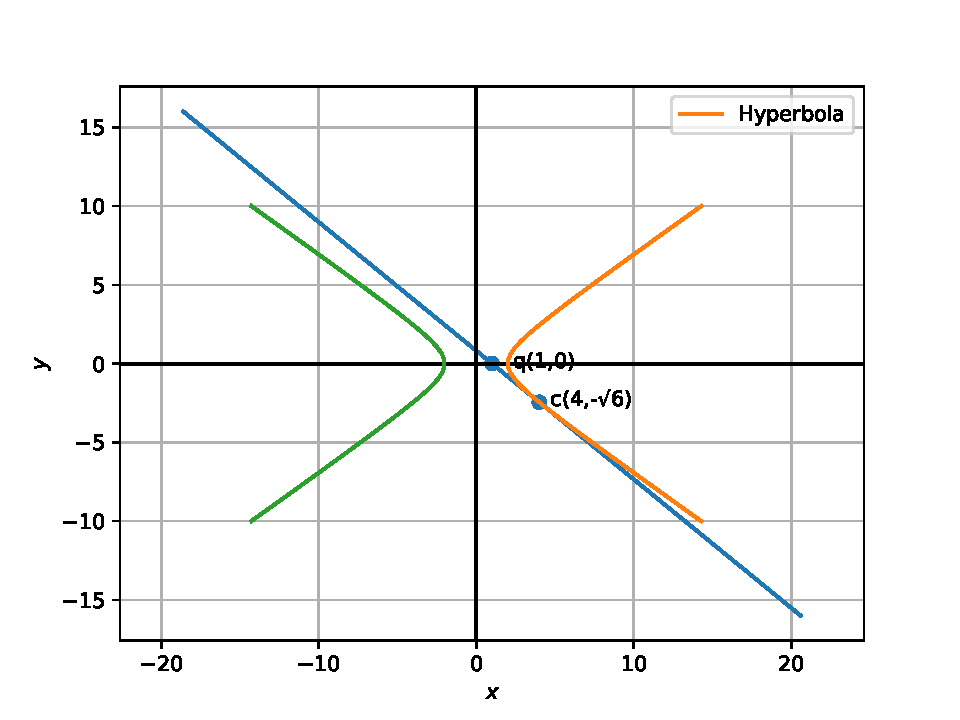
\includegraphics[width=1\columnwidth]{conics11.pdf}

\caption{}
\label{fig:parabola}
\end{figure}

The given equation of hyperbola $x^2-2y^2=4$ can be written in the general quadratic form as
\begin{align}
    \label{eq:conic_quad_form}
    \vec{x}^{\top}\vec{V}\vec{x}+2\vec{u}^{\top}\vec{x}+f=0
    \end{align}
where
\begin{align}
  \label{eq:V_matrix}
  \vec{V} &= \myvec{1 & 0\\0 & -1},
  \\
  \label{eq:u_vector}
  \vec{u} &= \myvec{0\\0},
  \\
  \label{eq:f_value}
  f &= -4
  %\\
\end{align}
The points of intersection of the line 
\begin{align}
  L: \quad \vec{x} = \vec{q} + \mu \vec{m} \quad \mu \in \mathbf{R}
\label{eq:conic_tangent}
\end{align}
with the conic section are given by
\begin{align}
\vec{x}_i = \vec{q} + \mu_i \vec{m}
\label{eq:conic_tangent_pts}
\end{align}
%
where
{\tiny
\begin{multline}
\mu_i = \frac{1}
{
\vec{m}^T\vec{V}\vec{m}
}
\lbrak{-\vec{m}^T\brak{\vec{V}\vec{q}+\vec{u}}}
\\
\pm
\rbrak{\sqrt{
\sbrak{
\vec{m}^T\brak{\vec{V}\vec{q}+\vec{u}}
}^2
-
\brak
{
\vec{q}^T\vec{V}\vec{q} + 2\vec{u}^T\vec{q} +f
}
\brak{\vec{m}^T\vec{V}\vec{m}}
}
}
\label{eq:tangent_roots}
\end{multline}
}



From the line $2x+\sqrt{6}y=2$ the vectors q,m are taken,
\begin{equation}
\vec{q}=\myvec{1\\0}
\end{equation}

\begin{equation}
\vec{m}=\myvec{-\sqrt{6}\\2}
\end{equation}

by substituting eq(2),(3),(4),(8),(9) in eq(7)
\begin{equation}
\mu = \frac{\sqrt{6}}{{2}}
\end{equation}
substituting eq(8),(9),(10) in eq(6) the point of contact is
\label{eq:conic_tangent_pts}
\begin{align}
\vec{c}= \vec{q}+ \mu \vec{m}
\label{eq:conic_tangent_pts}
\end{align}
\section*{\large Construction}

{
\setlength\extrarowheight{5pt}
\begin{tabular}{|l|c|}
    \hline 
    \textbf{Points} & \textbf{intersection points} \\ \hline
  $c$ & $\myvec{
   4\\
   -\sqrt{6}
   } $ \\\hline
  $q$ & $\myvec{
   1\\
   0
   } $ \\\hline
      \end{tabular}
}
\end{document}
